%-----------------------------------------------------------
%Background
\chapter{Background and similar projects}
\section{General background}
\par
Electronic data sharing has become an important tool in many scientific disciplines. This is especially true for those that work with large and complex data sets as. Thus, the value of data sharing has become increasingly apparent to scientists involved in neuroimaging for several reasons. The volume of data generated with brain imaging techniques is striking, and continues to be one of the most rapidly growing areas in this domain. Moreover, published findings reflect only a fraction of the data originally collected. The data themselves take a variety of forms and typically are not accessible for widespread sharing and use. Making neuroimaging data more accessible for sharing would facilitate the comparison of findings across laboratories.
\par
However, unlike fields in which databasing efforts have been successful, there are no universally accepted standards for the structure and content of neuroimaging data sets. Data formats vary widely across different laboratories and neuroimaging methods. This diversity of data and formats reflects several factors, including the rapid developments within the field and the rapid changes in our knowledge about brain. Indeed, neuroimaging methods are evolving quickly, and changes are sometimes accompanied by substantial changes in data content that directly affect  the format. For example, with the transition from anatomical to functional MRI, data formats changed from three to four dimensional. More critically, imaging of brain function demands a clear specification of the behavioral conditions under which the data were acquired. This is linked to the scientific hypotheses being tested. The number of potentially important behavioral variables is large and poorly defined.
\par
The figure 2.1 shows a part of the issues related to data sharing that need to be answered when researchers work on such projects.
\begin{figure}[!h]
\begin{center}
\includegraphics[scale=0.65]{images/database_issues.png}
\caption{\small Issues related to neuroimaging databases}
\end{center}
\end{figure}
\par
Faced to these issues and recognizing the increasing need for data sharing within the neuroimaging community, several groups have conducted researches to develop neuroimaging databases. Different models have been explored. Some use a centralized model that directly manages the storage and distribution of data. Others use a distribution model, in which a centralized listing is maintained that describes the available data and their location, whereas the data themselves are stored locally, under the control of their owner. The diversity of databases projects is a good thing to explore various approaches and to value each of them. In the next pages, we will review some of the most interesting projects conducted by team across the world, which proves the importance given to this research since several years. 

\section{The Human Imaging Database, by the BIRN}
\par
The Biomedical Informatics Research Network (BIRN) is a research American project launched in 2001 and supported by the National Institutes of Health's National Center for Research Resources (NCRR). It is one of the best known and complete work related to the sharing of data in the field of biomedical. It is composed by around 35 laboratories across the United States of America. The main goal of the projects is to propose a geographically distributed virtual community of shared resources associated with a large range of tools.
\par
As part of their huge work, the BIRN has been working on the Human Imaging Database (HID) which is an extensible database management system. It has been developed and implemented to address the problems associated with managing the increasingly large and diverse datasets collected as part of the morphometry and function BIRN (mBIRN, fBIRN) collaboratories. This system is comprised of three core components, among them, The Human Clinical and Imaging Database itself and an intuitive web based user interface.
\par
The database is composed of an extensible schema and structured core. The core database contains a hierarchical description of an experiment and how experimental protocols relate to this hierarchy. Then, the database at a particular site can be extended to contain relevant information concerning the research subjects used in an experiment, subjects assessments, the experimental data collected, the experimental protocols used and any annotation or statistics (metadata) normally included with an experiment. The database can be extended utilizing extended tuples which can be re-used and/or modified for other experiments. The complete system is used to manage and query local data at various research sites within BIRN. In addition to local operations, the system allows for mediated queries across multiple federated databases allowing researchers to discover data across all relevant sites. There are currently 12 federated HID databases, 11 Oracle and 1 PostgreSQL versions, storing clinical information.
\par
Regarding the user interface, the figure 2.2 shows his overall structure based on three tier Java 2 Enterprise Edition (J2EE) architecture. It consists of a client tier, a server/JSP based middle tier and a relational database based enterprise information source (EIS) tier. The EIS tier consists of the Human Clinical and Imaging Database and a collection of stored procedures/packages for low level data access functions. The middle tier currently consists of a web tier tier only. The underlying web application framework used for user interface is Jakarta Struts. It uses a controller servlet to intercept a web request and determine what to display next. The business logic layer is defined as the code manipulating business data (e.g. clinical assessments) relevant to the application. DAO is for Data Access Objects. Each software layer communicates with neighbor layers via well defined interfaces, which remain stable while the actual implementation can change drastically over time facilitating software maintenance and robustness.
\begin{figure}[!h]
\begin{center}
\includegraphics[scale=0.7]{images/birn.png}
\caption{\small Human Imaging Database Graphical User Interface structure\protect\footnotemark}
\end{center}
\end{figure}
\par
Thus, the projects conducted by the BIRN are very interesting in our case, especially the Human Imaging Database which provide a web-based interface and a relational database back-end for storing and managing brain imaging data. I will come back later on BIRN's works regarding the ontologies with NeuroLex (formerly BIRNLex).

\section{The Functional Magnetic Resonance Imaging Data Center}
\par
\footnotetext{Extracted from Ozyurt and al.,(2004) Web- accessible clinical data management within an extensible neuroimaging database. Society for Neuroscience, Washington, DC, 2005 Online}
The Functional Magnetic Resonance Imaging Data Center (fMRIDC) founded in 1999, has been thought to establish a facility for the sharing of functional neuroimaging data within the community of neuroscience. The Data Center has received during several years study data from fMRI analyses published in the Journal of Cognitive Neuroscience. Researchers exchange data with the Data Center through two simple means: contributing study data to the archive, in which researchers fill out detailed forms describing study protocols and individual subject information, and requesting study data from the record of studies in the repository.
\par
To address the problems associated with managing the increasingly large and diverse datasets collected, an object-relational database schema called Neurocore was developed. By exploiting the object-oriented properties of object-relational database technologies, Neurocore is a database architecture that is completely modifiable while maintaining a standard core structure.  Thus, this methodology can be used to extend the database to contain relevant information concerning the research subjects used in an experiment, the experimental data collected, the experimental protocols used and any annotations or statistics normally included with an experiment. The core database contains a hierarchical description of the experiment and how experimental protocols relate to this hierarchy. The ability to extend experimental descriptions in the database is accomplished through the use of object-relational technologies. This is very similar as the previous project (BIRN) exposed above.
\begin{figure}[!h]
\begin{center}
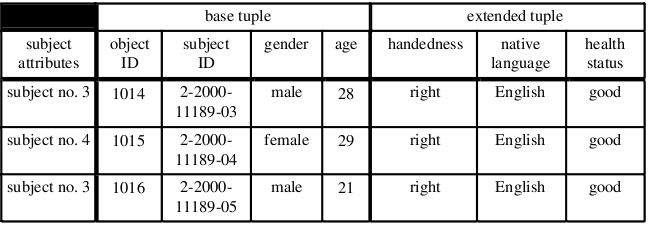
\includegraphics[scale=0.8]{images/fMRIDC_descriptor.png}
\caption{\small Descriptor ``subject'' in the database\protect\footnotemark}
\end{center}
\end{figure}
\footnotetext{Extracted from Van Horn, J.D., et al., The Functional Magnetic Resonance Imaging Data Center (fMRIDC): the challenges and rewards of large-scale databasing of neuroimaging studies, Science 356 (2001), 1323-1339}
\par
As shown in the figure 2.3, the inherent attributes for an entity constitute the ``base tuple'' that defines the minimum informational requirements for that entity. These base tuples can then be extended with additional attributes through the definition of an extended tuple. Furthermore, the extended tuples can be reused and/or modified for other experiments, and be used to guide future interactive data entry forms.
\par
Regarding the physical architecture of the fMRIDC computional resource, it is implemented in three tiers: the client Web browser (using HTML, XML, Java and Javascript), the web server running PHP and Python software and the database management system itself.
\begin{figure}[!h]
\begin{center}
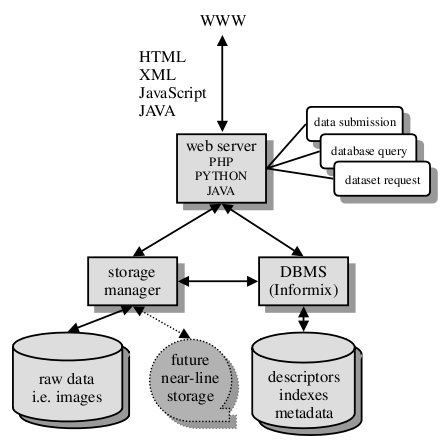
\includegraphics[scale=0.7]{images/fMRIDC_architecture.png}
\caption{\small Physical architecture of the fMRIDC\protect\footnotemark}
\end{center}
\end{figure}
\footnotetext{Extracted from Van Horn, J.D., et al., The Functional Magnetic Resonance Imaging Data Center (fMRIDC): the challenges and rewards of large-scale databasing of neuroimaging studies, Science 356 (2001), 1323-1339}
\par
Even if this project is relatively old compared to others presented here, it still remains very interesting by giving a specific structure for the overall system and by having specifics goals. Indeed, one of their main goal is to allow small and/or limited funded laboratories to access to a large bank of data in order to be able to reliably reproduced the fMRI results. Of course, they have implemented a very specific workflow to add data in the system in order to respect the human subject as well as the rights of the original authors. Unfortunately, the fMRIDC doesn't accept any new datasets but the others datasets can still be found on their website.
\section{The Computional Neuroscience Applications Research Infrastructure}
\section{The Extensible Neuroimaging Archive Toolkit}
\section{A work about other projects}






